\section{Tabelas} % (fold)
\label{sec:tabelas}

\subsection*{Introdução} % (fold)

\begin{frame}[fragile]
	
Utiliza-se a junção dos ambientes {\ttfamily table} para inserir as legendas e referências, com o {\ttfamily tabular} para inserir a tabela em si.

\begin{table}[htbp]
\caption{Opções para colunas}\centering\code
\begin{tabular}{|l|p{5cm}|}
\hline
l & Coluna justificada à esquerda \\ \hline
c & Coluna centralizada \\ \hline
r & Coluna justificada à direita \\ \hline
p\{'largura'\} & Texto alinhado verticalmente no inicio da célula \\ \hline
m\{'largura'\} & Texto alinhado verticalmente no meio da célula (requer pacote {\it array}) \\ \hline
b\{'largura'\} & Texto alinhado verticalmente na base da célula (requer pacote {\it array}) \\ \hline
| & linha vertical \\ \hline
|| & linha vertical dupla \\ \hline
\end{tabular}
\end{table}

\end{frame}


\subsection*{Código} % (fold)
\label{sub:c_digo}

\begin{frame}{Exemplo para a \nameref{tab:exemplo}}
\lstinputlisting[linewidth=10cm]{tables/table.tex}
\begin{table}[h]
	\caption{Tabela de Exemplo}
	\begin{tabular}{l|c|l||r||p{3cm}}
		0 & 1 & Texto & 3 & Texto muito longo para célula\\
		4 & Texto & 7 & $\int_0^1 2x dx$ & 9 \\ \hline
		&  & $\partial$ &  &
	\end{tabular}
	\label{tab:exemplo}
\end{table}

\end{frame}

\subsection{Ferramentas}
\begin{frame}{Ferramentas Online}
	
\begin{figure}[htbp!]
	\centering
	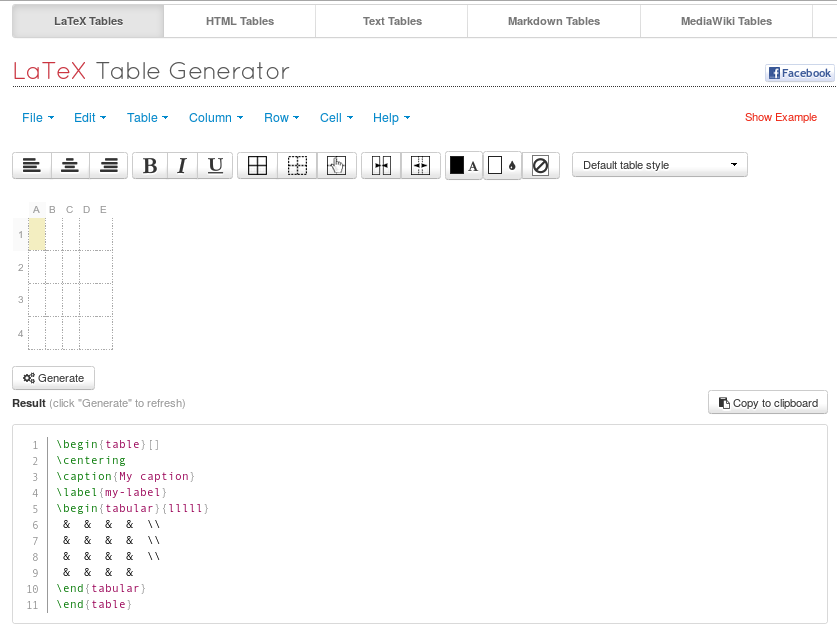
\includegraphics[width=0.9\textwidth]{figuras/table_online.png}
	\caption{ }
	\label{fig:tableOnline}
\end{figure}

\end{frame}

\begin{frame}{LibreOffice~-~Calc}
\begin{figure}[htbp!]
	\centering
	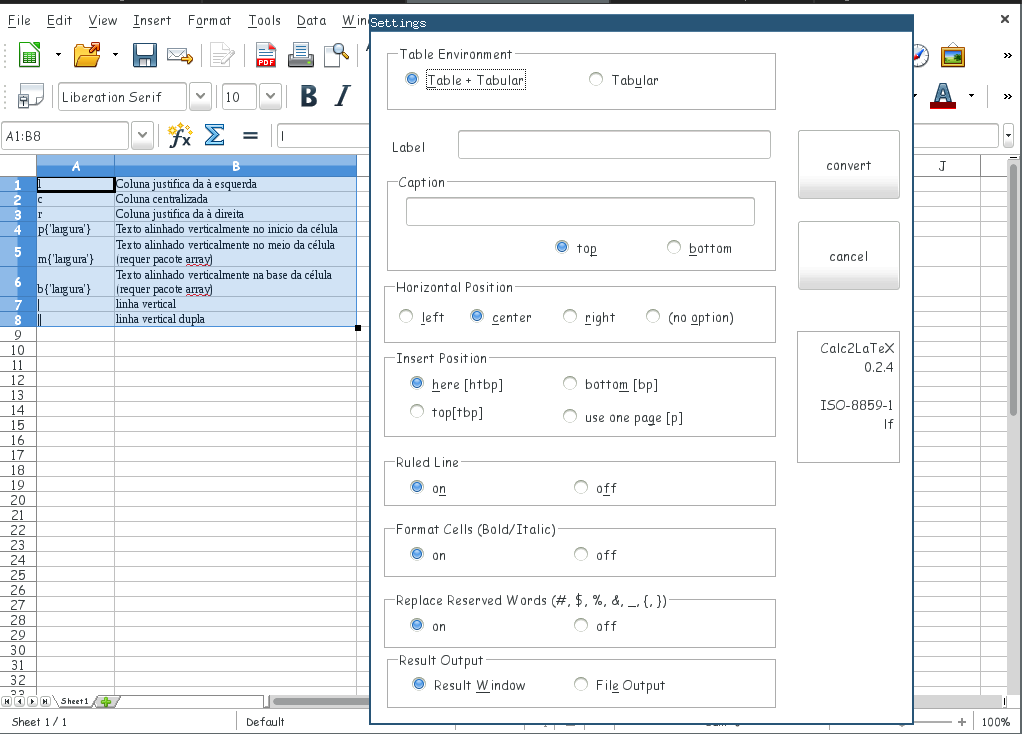
\includegraphics[width=0.9\textwidth]{figuras/calc1.png}
	\caption{ }
	\label{fig:tableOnline}
\end{figure}
\end{frame}

\begin{frame}{LibreOffice~-~Calc}
\begin{figure}[htbp!]
	\centering
	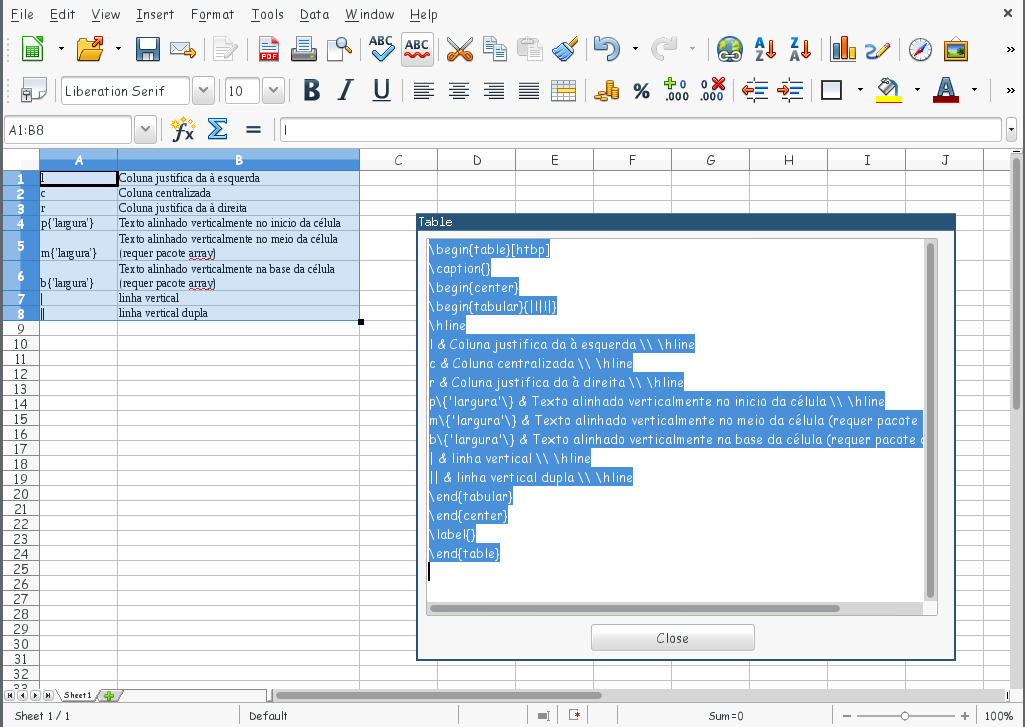
\includegraphics[width=0.9\textwidth]{figuras/calc2.png}
	\caption{ }
	\label{fig:tableOnline}
\end{figure}
\end{frame}